%% utricularia.tex
%% Author: Leighton Pritchard
%% Copyright: James Hutton Institute
%% Example slides: Comparative Genomics In The News 2015

%
\begin{frame}
  \frametitle{Comparative genomics in the news
                   \footnote{\tiny{\href{http://www.washingtonpost.com/news/speaking-of-science/wp/2015/02/23/the-mysterious-genes-of-carnivorous-bladderwort-reveal-themselves/
}{Washington Post 23/2/2015
}}}
                   \footnote{\tiny{\href{http://dx.doi.org/10.1038/nature12132
}{Ibarra-Laclette \textit{et al}. (2013) \textit{Nature} doi:10.1038/nature12132
}}}
                   \footnote{\tiny{\href{http://dx.doi.org/10.1093/molbev/msv020
}{Carretero-Paulet \textit{et al}. (2015) \textit{Mol. Biol. Evol.} doi:10.1093/molbev/msv020
}}}
}
    \begin{columns}[c] 
      \column{.6\textwidth} 
        \begin{itemize}
          \item \textcolor{RawSienna}{\textit{Utricularia gibba}: carnivorous bladderwort}
          \item \textcolor{hutton_blue}{Genome: 82Mbp, 17,324 genes \\
          (wheat: 17bn bases, $\approx$94-96k genes)}
          \item Intergenic region contraction \\
          (3\% repeat elements; most plants: 10-60\% repeat elements)
          \item \textcolor{hutton_green}{Genomic context for flowering plants does not require ``hidden regulators'' (cf. ENCODE)}
        \end{itemize}
      \column{.4\textwidth}
        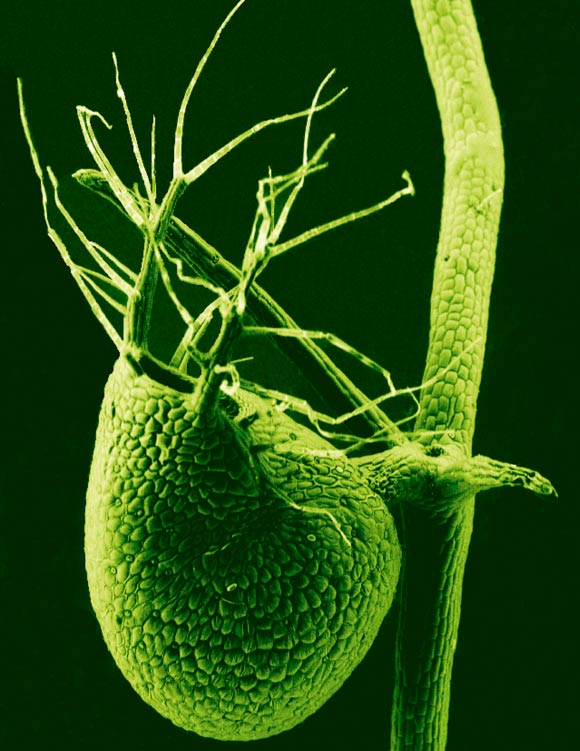
\includegraphics[height=0.3\textheight]{images/Utricularia-gibba}
        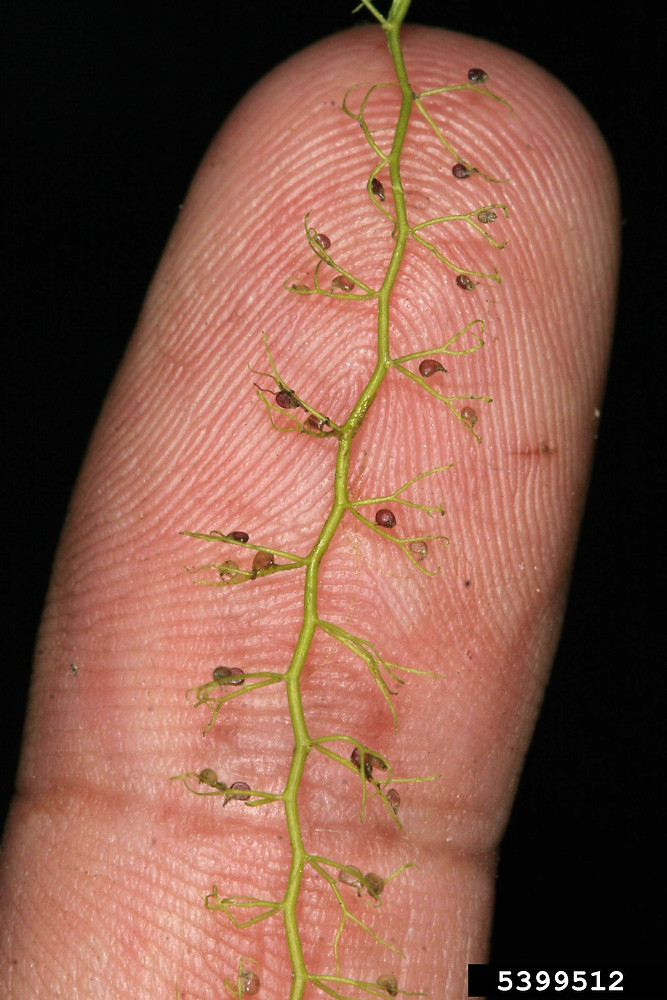
\includegraphics[height=0.3\textheight]{images/utricularia-gibba-finger} \\
        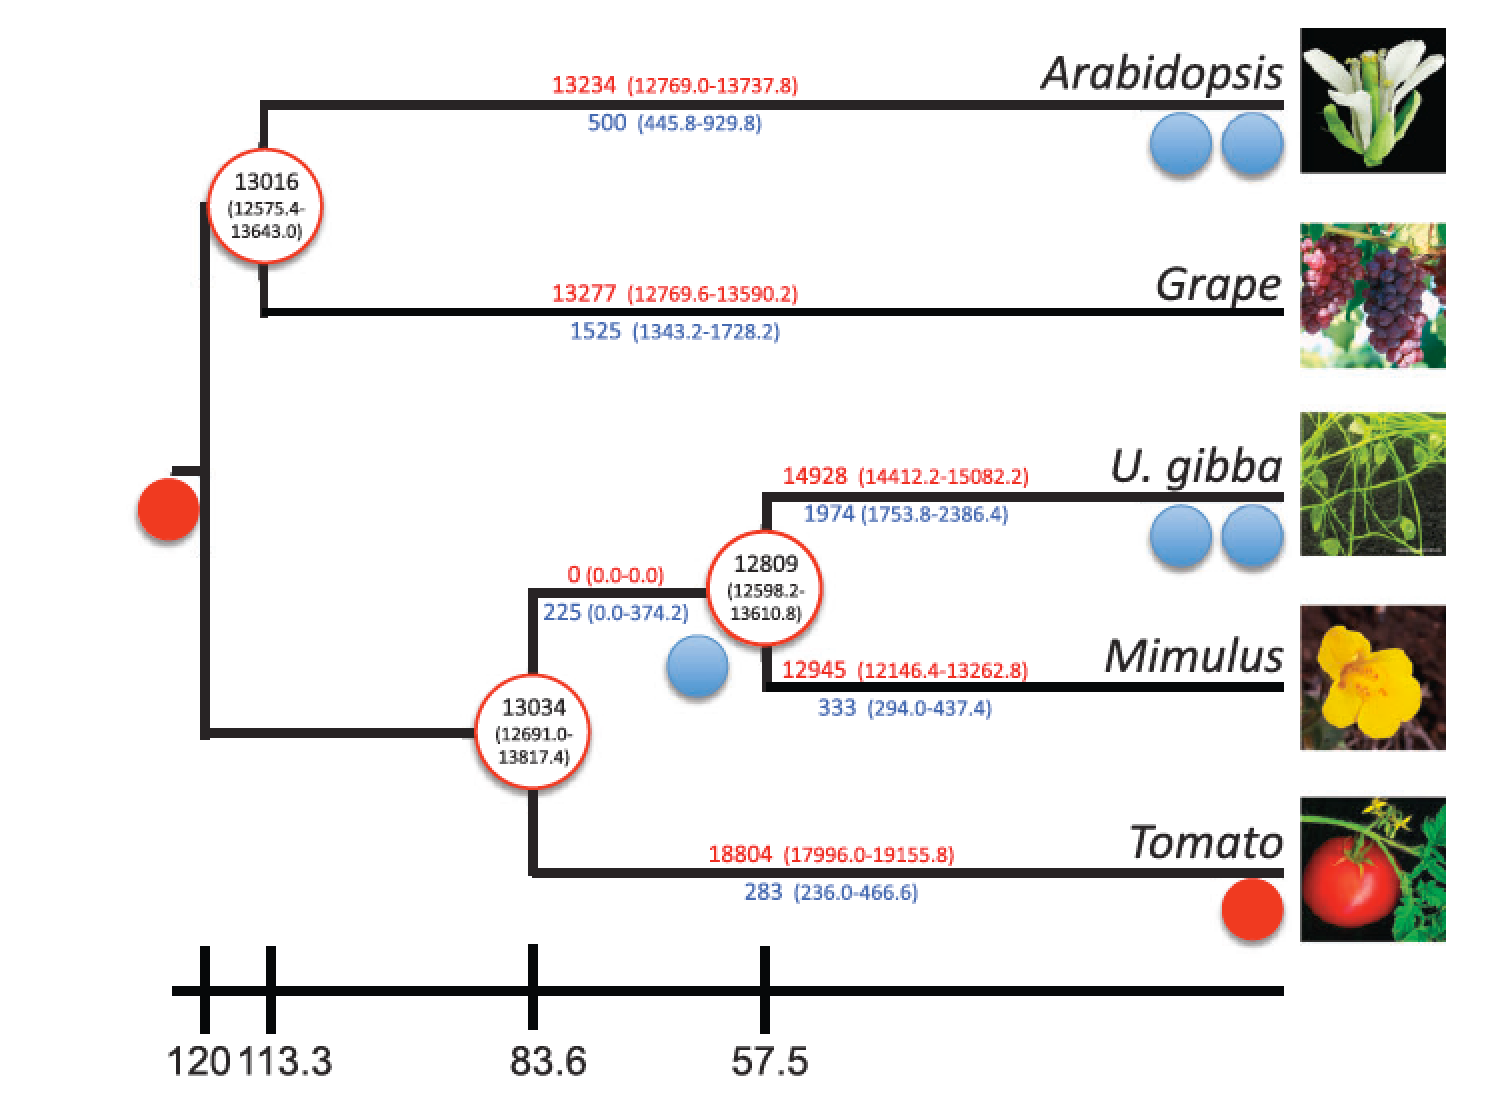
\includegraphics[width=\textwidth]{images/U_gibba_tree}        
    \end{columns}  
\end{frame}